\documentclass[11pt]{article}

\usepackage[letterpaper]{geometry}
%\usepackage[letterpaper,left=2.5cm,top=2cm,right=2.5cm,bottom=2cm]{geometry}

\usepackage[utf8]{inputenc}
\usepackage{mathpazo}
\usepackage{amsmath}
\usepackage{amsfonts}
\usepackage{physics}
\usepackage{siunitx}

\usepackage{fancyhdr}

\usepackage{graphicx}
\usepackage{float}

\usepackage[shortlabels,inline]{enumitem}

% Hyperlinks with decent looking default colors.
\usepackage{hyperref}
\usepackage{xcolor}
\hypersetup{
  colorlinks,
  linkcolor={red!50!black},
  citecolor={blue!50!black},
  urlcolor={blue!80!black}
}

% For those sexy spaced low small caps from classic-thesis!
\usepackage{microtype}
\usepackage{textcase}
\DeclareRobustCommand{\spacedlowsmallcaps}[1]{%
  \textls[80]{\scshape\MakeTextLowercase{#1}}%
}

\pagestyle{fancy} 
\fancyhead{}
\rhead{\spacedlowsmallcaps{Ali Ramadhan}}
\lhead{\spacedlowsmallcaps{12.818: Project one}}

\title{\spacedlowsmallcaps{\small 12.818: Introduction to Atmospheric Data and Large-scale Dynamics}\\ \spacedlowsmallcaps{\large Project one: Surface and upper air observations}}
\author{Ali Ramadhan}
\date{\today}

\renewcommand\thesection{\Alph{section}}

\begin{document}
\chead{}
\cfoot{\thepage}
\renewcommand{\headrulewidth}{0pt}

\maketitle

\section{Map of surface observations}
\subsection*{Surface map}
Figure \ref{fig:surfaceMap} shows a surface weather map center over Boston, MA (BOS). The surface air temperature is \SI{69}{\SIUnitSymbolDegree\F} while the green the dew point is \SI{68}{\SIUnitSymbolDegree\F}. Since the dew point is so close to the actual air temperature, the air is almost maximally saturated with water vapor and the relative humidity is close to $100\%$. This seems to be the case for most of southern New England, leading the water to condense and form a thin fog being over much of the area except for some light rain along the Massachusetts-New Hampshire border by Nashua. The moisture was brought in as the remnants of hurricane Irma passed through the region bringing with it warmer moisture-rich air from the tropics. The cyan number above the station code is the pressure at sea-level, reported in tenths of hectopascals (\SI{}{\hecto\Pa}), with the leading 10 or 9 omitted, thus the $161$ corresponds to a pressure of \SI{1016.1}{\hecto\Pa}. The white arrow indicates that winds are blowing \emph{from} the south with a speed of approximately \SI{5}{\knot}.

\begin{figure}
  \centering
  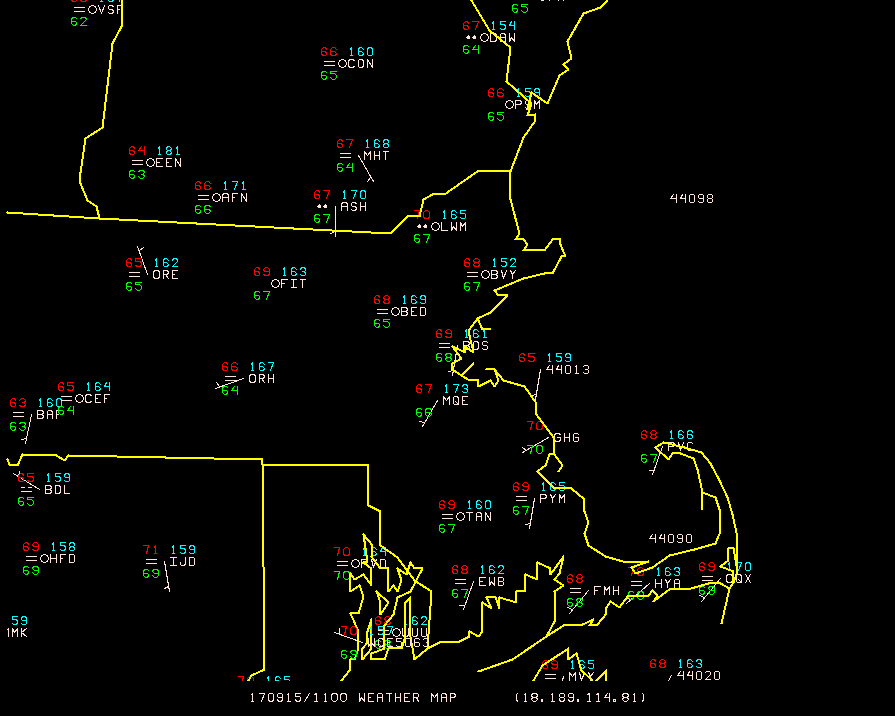
\includegraphics[width=\textwidth]{surfaceMapBOS.png}
  \caption{Surface weather map of Massachusetts and bordering states centered on Boston, MA, and taken on September 15, 2017 at 11:00 UTC (07:00 EST).}
  \label{fig:surfaceMap}
\end{figure}

Plymouth (PYM) and Worcester (ORH) are both also experiencing similar foggy conditions. The temperature at Plymouth is \SI{69}{\SIUnitSymbolDegree\F} with a dew point of \SI{67}{\SIUnitSymbolDegree\F} and a pressure of \SI{1016.5}{\hecto\Pa} with winds blowing from the south with a speed of \SI{5}{\knot}. The temperature at Worcester is \SI{66}{\SIUnitSymbolDegree\F} with a dew point of \SI{64}{\SIUnitSymbolDegree\F} and a pressure of \SI{1016.7}{\hecto\Pa} with winds blowing from the southeast with a speed of \SI{5}{\knot}.

\subsection*{Surface meteogram}
Figure \ref{fig:meteogram} shows a surface meteogram for Boston, MA for the eleven or so hours leading up to the morning of September 15, 2017. We see that the temperature dropped slightly overnight while the dew point rose overnight, increasing the humidity and leading to the formation of a light fog around 07:00 EST. However, with the sun out temperatures will probably increase and the fog will dissapate quickly.

\begin{figure}
  \centering
  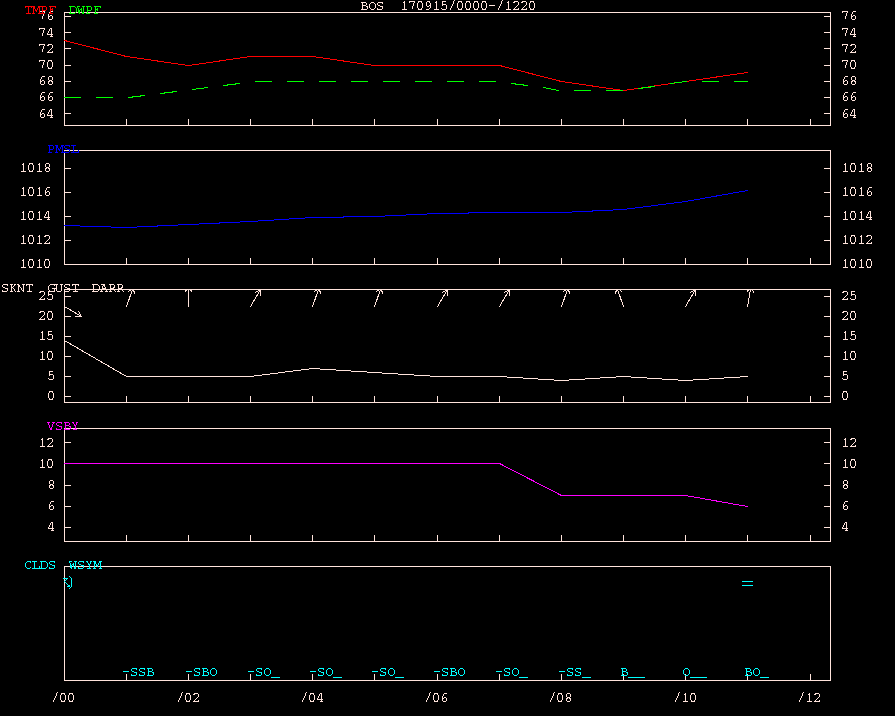
\includegraphics[width=\textwidth]{meteogramBOS.png}
  \caption{Surface meteogram of Boston, MA showing surface air temperature, dew point, surface pressure, wind speed, visibility, and weather observations for September 15, 2017 from 00:00--11:20 UTC (20:00--07:20 EST).}
  \label{fig:meteogram}
\end{figure}

The surface pressure slightly rose overnight as well from \SI{1013}{\hecto\Pa} to \SI{1016.7}{\hecto\Pa} and is still rising. Last night, light winds of \SI{15}{\knot} from the northwest calmed to a constant \SI{5}{\knot} wind blowing from the southwest throughout the night with no gusts. Visibility last night was a clear \SI{10}{miles} with a drop to \SI{7}{miles} due to more humid conditions and a further drop to \SI{6}{miles} with the light fog coming in.

We can see that a mild thunderstorm passed last night followed by low-lying scattered clouds and broken clouds high up, as expected. The higher clouds turned to overcast for a bit and moved along while the scattered clouds remained over much of the night as the storm passed through the area before turning to broken then overcast as the fog developed. The passing of the thunderstorm may be the reason for the rising surface pressures experienced overnight.

\section{Map of upper air observations}
Figures \ref{fig:radiosonde850hPa}--\ref{fig:radiosonde250hPa} show upper air radiosonde observations for the United States and Canada at geopotential heights of \SIlist{850; 500; 250}{\hecto\Pa} respectively.

At \SI{850}{\hecto\Pa} (roughly \SI{1500}{\m}), we see that the air temperature has dropped considerably by about \SI{55}{\SIUnitSymbolDegree\F}, now below freezing everywhere. The wind speeds above New England remain roughly the same speed and we can see some stronger \SI{25}{\knot} southernly winds above the southern Great Plains.

At \SI{500}{\hecto\Pa} (roughly \SI{5.7}{\km}), temperatures have now dropped by roughly \SI{80}{\SIUnitSymbolDegree\F} compared to surface temperatures. Winds above New England remain calm and we see stronger westerly winds above the southern Atlantic states. Easterly winds are starting to appear from coast to coast above the Canadian provinces, representing the polar jet stream.

At \SI{250}{\hecto\Pa} (roughly \SI{10.5}{\km}), temperatures have dropped a total of approximately \SI{115}{\SIUnitSymbolDegree\F} compared to surface temperatures and the wind directions have remained roughly the same but have strengthened. In general, winds get stronger from the surface up to a geopotential height of \SI{250}{\hecto\Pa} as there are no land boundaries in place to slow down the circulation of the atmosphere.

\begin{figure}
  \centering
  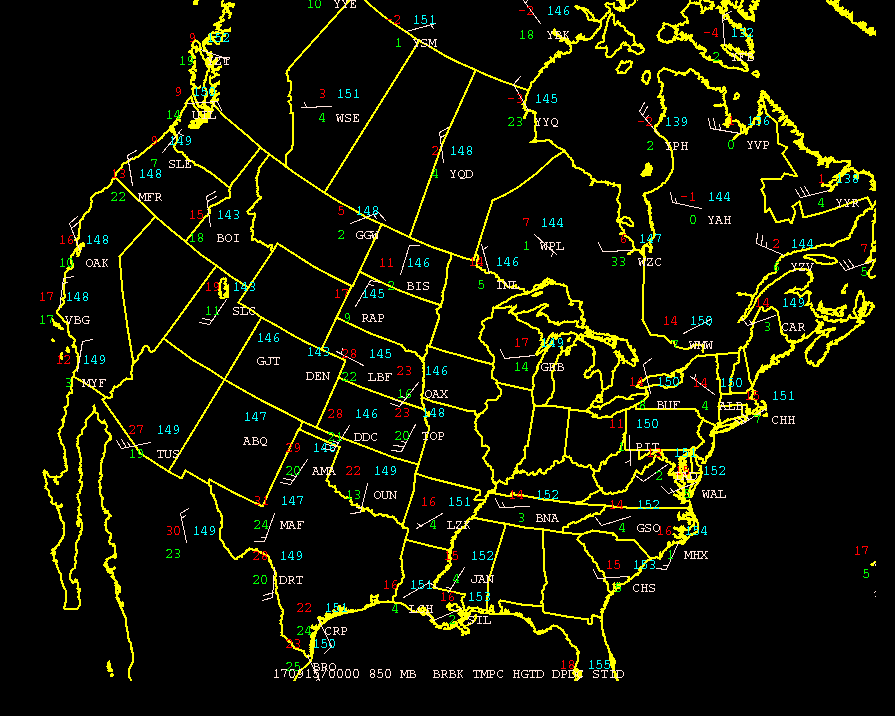
\includegraphics[width=\textwidth]{radiosondeUSA850hPa.png}
  \caption{Upper air radiosonde observations for the continental United States and Canada at a geopotential height of \SI{850}{\hecto\Pa} on September 15, 2017 00:00 UTC (September 14, 2017 00:00 EST).}
  \label{fig:radiosonde850hPa}
\end{figure}

\begin{figure}
  \centering
  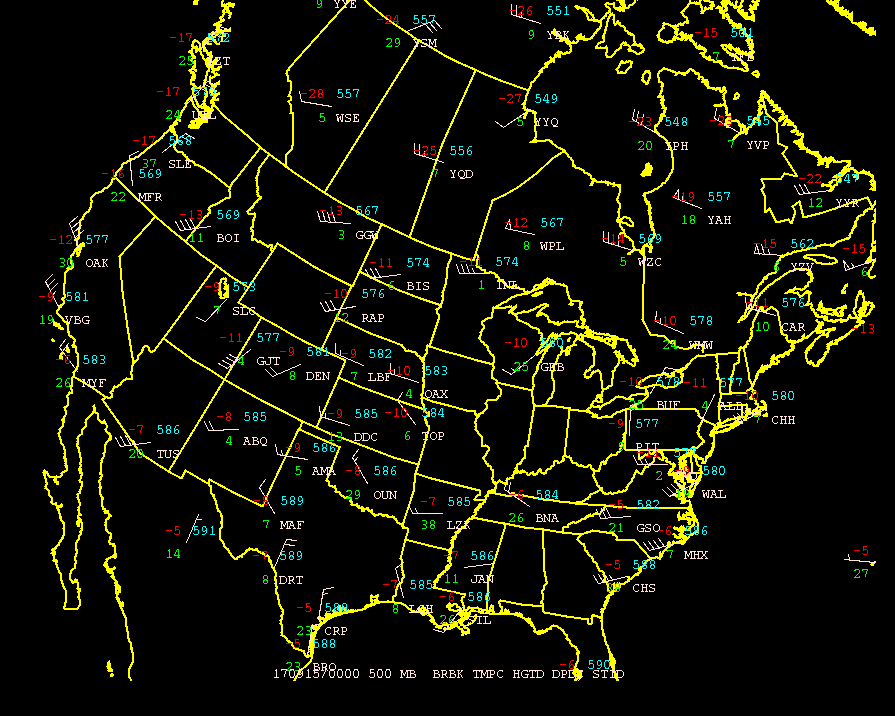
\includegraphics[width=\textwidth]{radiosondeUSA500hPa.png}
  \caption{Upper air radiosonde observations for the continental United States and Canada at a geopotential height of \SI{500}{\hecto\Pa} on September 15, 2017 00:00 UTC (September 14, 2017 00:00 EST).}
  \label{fig:radiosonde500hPa}
\end{figure}

\begin{figure}
  \centering
  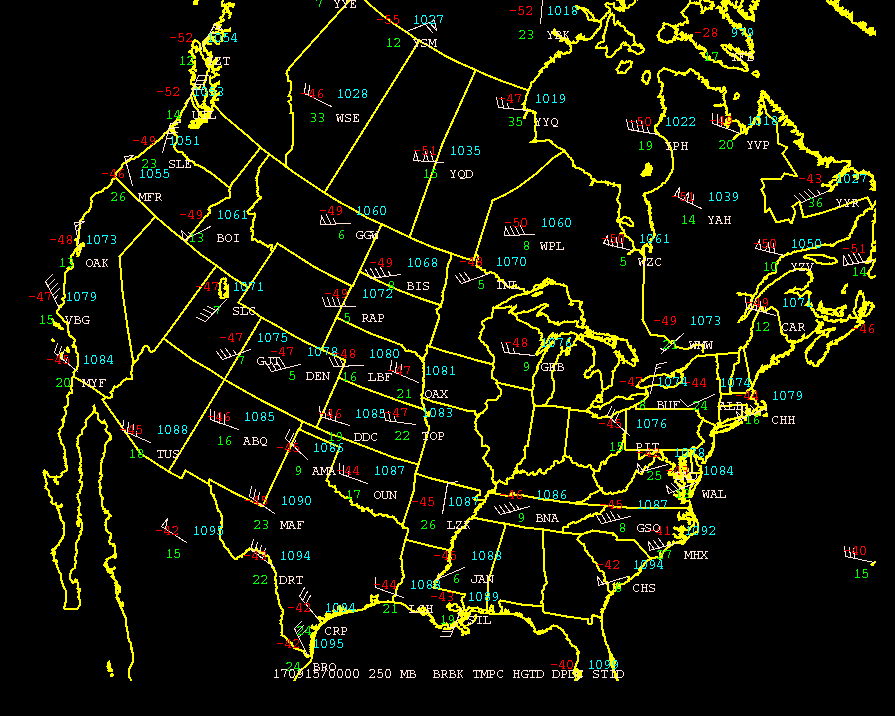
\includegraphics[width=\textwidth]{radiosondeUSA250hPa.png}
  \caption{Upper air radiosonde observations for the continental United States and Canada at a geopotential height of \SI{250}{\hecto\Pa} on September 15, 2017 00:00 UTC (September 14, 2017 00:00 EST).}
  \label{fig:radiosonde250hPa}
\end{figure}

\end{document}